% !TeX spellcheck = <none>
%testtest
\section{Background}
%Checklist Preface: https://www.scribbr.com/dissertation/preface-dissertation/

 

\paragraph{Production line}

The production line located at \ac{IPKW} in the \ac{MIC} building is being developed by the \ac{SPC}. The production line will produce steering knuckles made of \ac{FRP}. To compete in the future developements of "Smart Manufacturing", \textit{the Smart Cell  project investigates on an automated production cell for the realization of structural composite components which must be produced in large scale or mass produced} (see \cite{SPCWebsite}). %, Smart-Cell project description). 


%\paragraph{Definition of a Robot}
%%% definition/clickbait
%Robots \cite{robotDef} can be defined as programmable movement automatons \cite{automatonDef} that can perform tasks without human supervision and can be taught at least repetitive tasks. 
%Increasingly, also ways to sense their surroundings are added to improve their movements according to the situation \cite{robotDef2}. 
%These sensors are placed additionally to the standard feedback-control sensors like pulse encoders and allow the robot to handle a wider range of situations without human intervention. % at their axes to feedback control their endpoint position accuracy. 
%%system supervision - robotic system - 
%% A robot is defined as a programmable movement automaton, with the ability to perform tasks without human supervision. Not only can the robot be taught repetitive tasks, that it can execute with pulse encoders at their axes. it can as well sense its surroundings and on the basis of that information improve movements accordingly. 
%% go to old from new! Go from general to specific Don't jump from general to specific to examples, don't mix it because reader has then to do all the work. and show that you are not only able to understand concepts, but are able to 1) present them in a coherent way and (later) critique them. chronology
%\medskip


\paragraph{Origin of robots}
The term \gls{Robot} was first mentioned 1920 by Karel \v{C}apek in a  1920 Czech science fiction play "Rossum’s Universal Robots” and means serf labor but colloquially means hardwork or drudgery \cite{CorkeRoboticVisionControl}. With the upscaling of production in the past century, industrial \glspl{Robot} were developed to do work, that was too repetitive, dangerous or difficult for workers. The first patent for robots was filed in 1954 by George C. Devol. It was a mechanical arm with a gripper, mounted on a track. %Motion sequences were encoded as magnetic patterns on predecessors of harddrives. 
Unimation, founded by Devol and Joseph Engelberger in 1956 installed their first industrial robot Unimate, shown in \Autoref{fig:Unimate}, in 1961.


% is well documented in "Robotics, Vision and Control: Fundamental Algorithms in MATLAB" by Peter Corke \cite{CorkeRoboticVisionControl}:
%%From Corce Robotics Toolbox: (Refactor!)
%\textit{The term robot first appeared in a 1920 Czech science fiction play "Rossum’s Universal Robots” by Karel \v{C}apek (pronounced Chapek). 
%The term was coined by his brother Josef, and in the Czech language means serf labor but colloquially means hardwork or drudgery. 
%The robots in the play were artificial people or androids and as in so many robot stories that follow this one, the robots rebel and it ends badly for humanity. 
%Isaac Asimov’s robot series, comprising many books and short stories written between 1950 and 1985, explored issues of human and robot interaction and morality. 
%The robots in these stories are equipped with “positronic brains” in which the “Three laws of robotics” are encoded. These stories have influenced subsequent books and movies which in turn have shaped the public perception of what robots are. 
%The mid twentieth century also saw the advent of the field of cybernetics  – an uncommon term today but then an exciting science at the frontiers of understanding life and creating intelligent machines.
%The first patent for what we would now consider a robot was filed in 1954 by George C. Devol and issued in 1961. 
%The device comprised a mechanical arm with a gripper that was mounted on a track and the sequence of motions was encoded as magnetic patterns stored on a rotating drum. 
%The first robotics company, Unimation, was founded by Devol and Joseph Engelberger in 1956 and their first industrial robot shown in [ Fig. \ref{fig:Unimate} ] was installed in 1961.} 

\begin{figure}[H]
	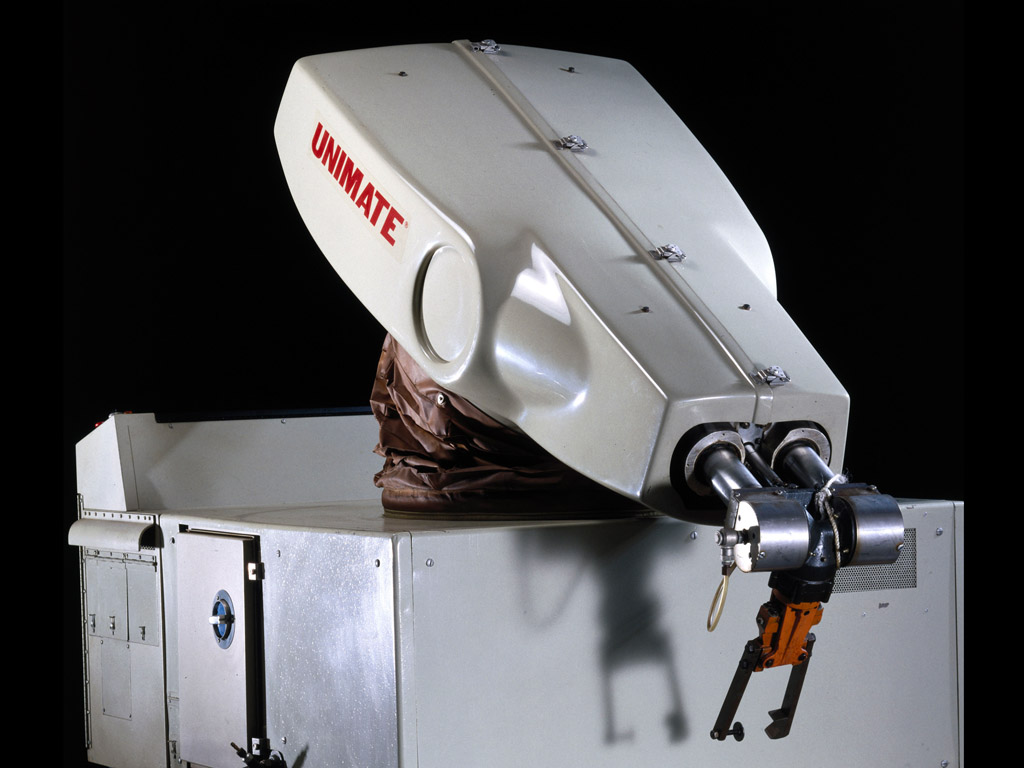
\includegraphics[
	width=0.5\linewidth,
	center,
	keepaspectratio,
	]{Unimate}
	\caption{Unimate, the grandfather of industrial robots \cite{UnimateIEEE}  }
	\label{fig:Unimate}
\end{figure}
%(Unimation) (Get picture from children book)
\medskip



\paragraph{Simple robots}
%% simple robots
%I have started working with robots and robotic systems in my bachelor studies. 
%As a starting engineer, I was exploring the possibilities of
CNC mills and 3D printers allow automated manufacturing with varying degrees of precision and speed.
These are very simplistic robotic systems based on a feedforward control with stepper motors for position control. 
For starting a production process, these devices need to be calibrated and the position and orientation are taught by pointing the drill/printing head to the markerpoints manually. 
As no feedback control is usually available on these devices, loss of step control and other errors are possible and can go unnoticed until the end of production, when the part is inspected.
\medskip


\paragraph{Current robots}
%% current robots
Highly developed automated platforms like the Fanuc 210F have feedback-sensors and -control for point to point as well as tracking motion, computer vision as seen on the deltarobot at \ac{SPC} (see \Autoref{sec:Deltarobot}), digital and analog I/O,  builtin- safety like the \ac{DCS} motion safety system and high speed fieldbus connectivity like Profinet.
With a teach pendant, these Robots can be configured and programmed. Alternatively, \ac{PC}-based proprietary manufacturer-specific software like Roboguide with a model based test cell can be used to program the robot. 
\medskip

\paragraph{Future robots}
%% future robot (envisioned)
%To compete in the future developements of "Smart Manufacturing", \textit{the Smart Cell  project investigates on an automated production cell for the realization of structural composite components which must be produced in large scale or mass produced} (see \cite{SPCWebsite}, Smart-Cell project description). 
Within research in materials and production, the automation environment system is of interest for this research.
To manage the interaction between material but also the machines among each other, a \ac{DDS} couples the subsystems as a middleware as seen in \Autoref{fig:SmartCellDDS}. A middleware is "glue code" that helps to interface systems with each other to exchange commands and data to use it as a single robotic system. 
\ac{ROS} is a proposed middleware to model, simulate, and control the production line as a homogenious distributed system. 
Besides the classical publish subscribe  pattern to simplify network programming, \ac{ROS} provides an ecosystem of interchangeable nodes and drivers with a wide codebase for complex tasks.
\medskip
\begin{figure}[H]
	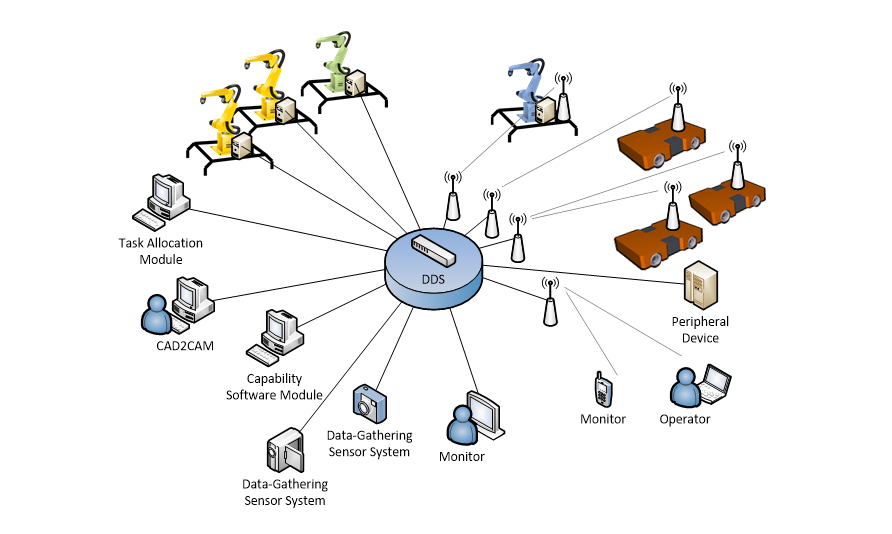
\includegraphics[
	width=0.95\linewidth,
	center,
	keepaspectratio,
	]{SmartCellDDS}
	\caption{\ac{DDS} as central information exchange platform}
	\label{fig:SmartCellDDS}
\end{figure}

%What are keywords for each of the paragraphs? e.g. HUMAN supervision, robotic Systems, etc..
%Use strong Verbs!
%signalwords
%
